\documentclass[11pt]{article}
\usepackage[margin=1in]{geometry}
\usepackage{graphicx}
\usepackage{hyperref}
\usepackage{enumitem}
\setlist{nosep}

\title{OLD Data Centers in Spain: Mapping Existing Facilities and Context}
\author{}
\date{March 2026}

\begin{document}
\maketitle

\section*{Overview}
This note summarizes the work completed in the R notebook \texttt{DataCenters\_Current\_Map.rmd} and
aligns it with the broader project context documented in \texttt{dataCenters.ipynb}. The core goal is
to map existing data centers in Spain and situate them within the provincial geography used for the
analysis of environmental and infrastructure stress at the NUTS3 (52 provinces) scale.

\section*{Why This Matters (Project Context)}
The broader research question in \texttt{dataCenters.ipynb} is whether predicted or likely data center
development in Spain concentrates in provinces already under compound environmental stress
(water scarcity, heat extremes, and land-use pressure). If high-suitability provinces coincide with
high-stress provinces, new data center development risks intensifying already strained resources
such as water for cooling, land footprint, and grid capacity. The provincial (NUTS3) scale is used
because it is the finest spatial unit with consistent economic and environmental statistics.

\section*{Data Sources and Scraping (from \texttt{dataCenters.ipynb})}
\begin{itemize}
  \item \textbf{Directory source:} \texttt{datacentermap.com/spain} is used as the main public directory
  of data centers in Spain.
  \item \textbf{Scraping approach:} the Spain index page is crawled to enumerate all region subpages,
  then each region page is scraped to extract individual facility records (operator, city, region, and
  available facility metadata).
  \item \textbf{Geocoding:} facility locations are geocoded using Nominatim (OpenStreetMap) with rate
  limiting (a 10-second delay between requests).
  \item \textbf{Outputs:} the notebook writes facility records to \texttt{data/datacentermap\_spain.csv}
  and \texttt{data/dc\_locations.geojson} (used downstream in the analysis).
\end{itemize}

\section*{Administrative Base Layer (52 Provinces)}
The analysis adopts Spain's 52 provinces (NUTS3) as the standard spatial unit. The project notebook
references GADM v4.1, Level 2 (Spain provinces) as the boundary source and notes that it is the most
appropriate level for consistent provincial statistics.

\begin{figure}[ht]
  \centering
  \fbox{\parbox{0.95\textwidth}{
    \textbf{Map 1 placeholder: Spain, 52 provinces (NUTS3).}
    \newline
    Add the province boundary map here (GADM v4.1 Level 2 or GISCO NUTS3) so this figure displays the
    full 52-province base layer before the data center overlay.
  }}
  \caption{Spain provinces (NUTS3, 52 total).}
\end{figure}

\section*{R Notebook Workflow (\texttt{DataCenters\_Current\_Map.rmd})}
The R notebook performs the following steps:
\begin{itemize}
  \item Loads packages for spatial handling and visualization (\texttt{sf}, \texttt{ggplot2},
  \texttt{rnaturalearth}, \texttt{giscoR}, \texttt{dplyr}).
  \item Reads the cleaned data center list from \texttt{data/spain\_datacenters\_v2.xlsx}.
  \item Filters out records without valid latitude/longitude.
  \item Categorizes facilities by reported size (m\textsuperscript{2}) into five bins:
  \texttt{>100,000}, \texttt{10,000--100,000}, \texttt{1,000--10,000}, \texttt{<1,000}, and
  \texttt{Unknown}.
  \item Generates a national map of Spain with data centers symbolized by size category and saves
  the output to \texttt{outputs/data\_center\_map.jpg}.
  \item Produces a focused map of the Comunidad de Madrid (NUTS3 ES300) and saves it to
  \texttt{outputs/madrid\_dc\_map.jpg}.
\end{itemize}

\section*{Key Graphics}
\begin{figure}[ht]
  \centering
  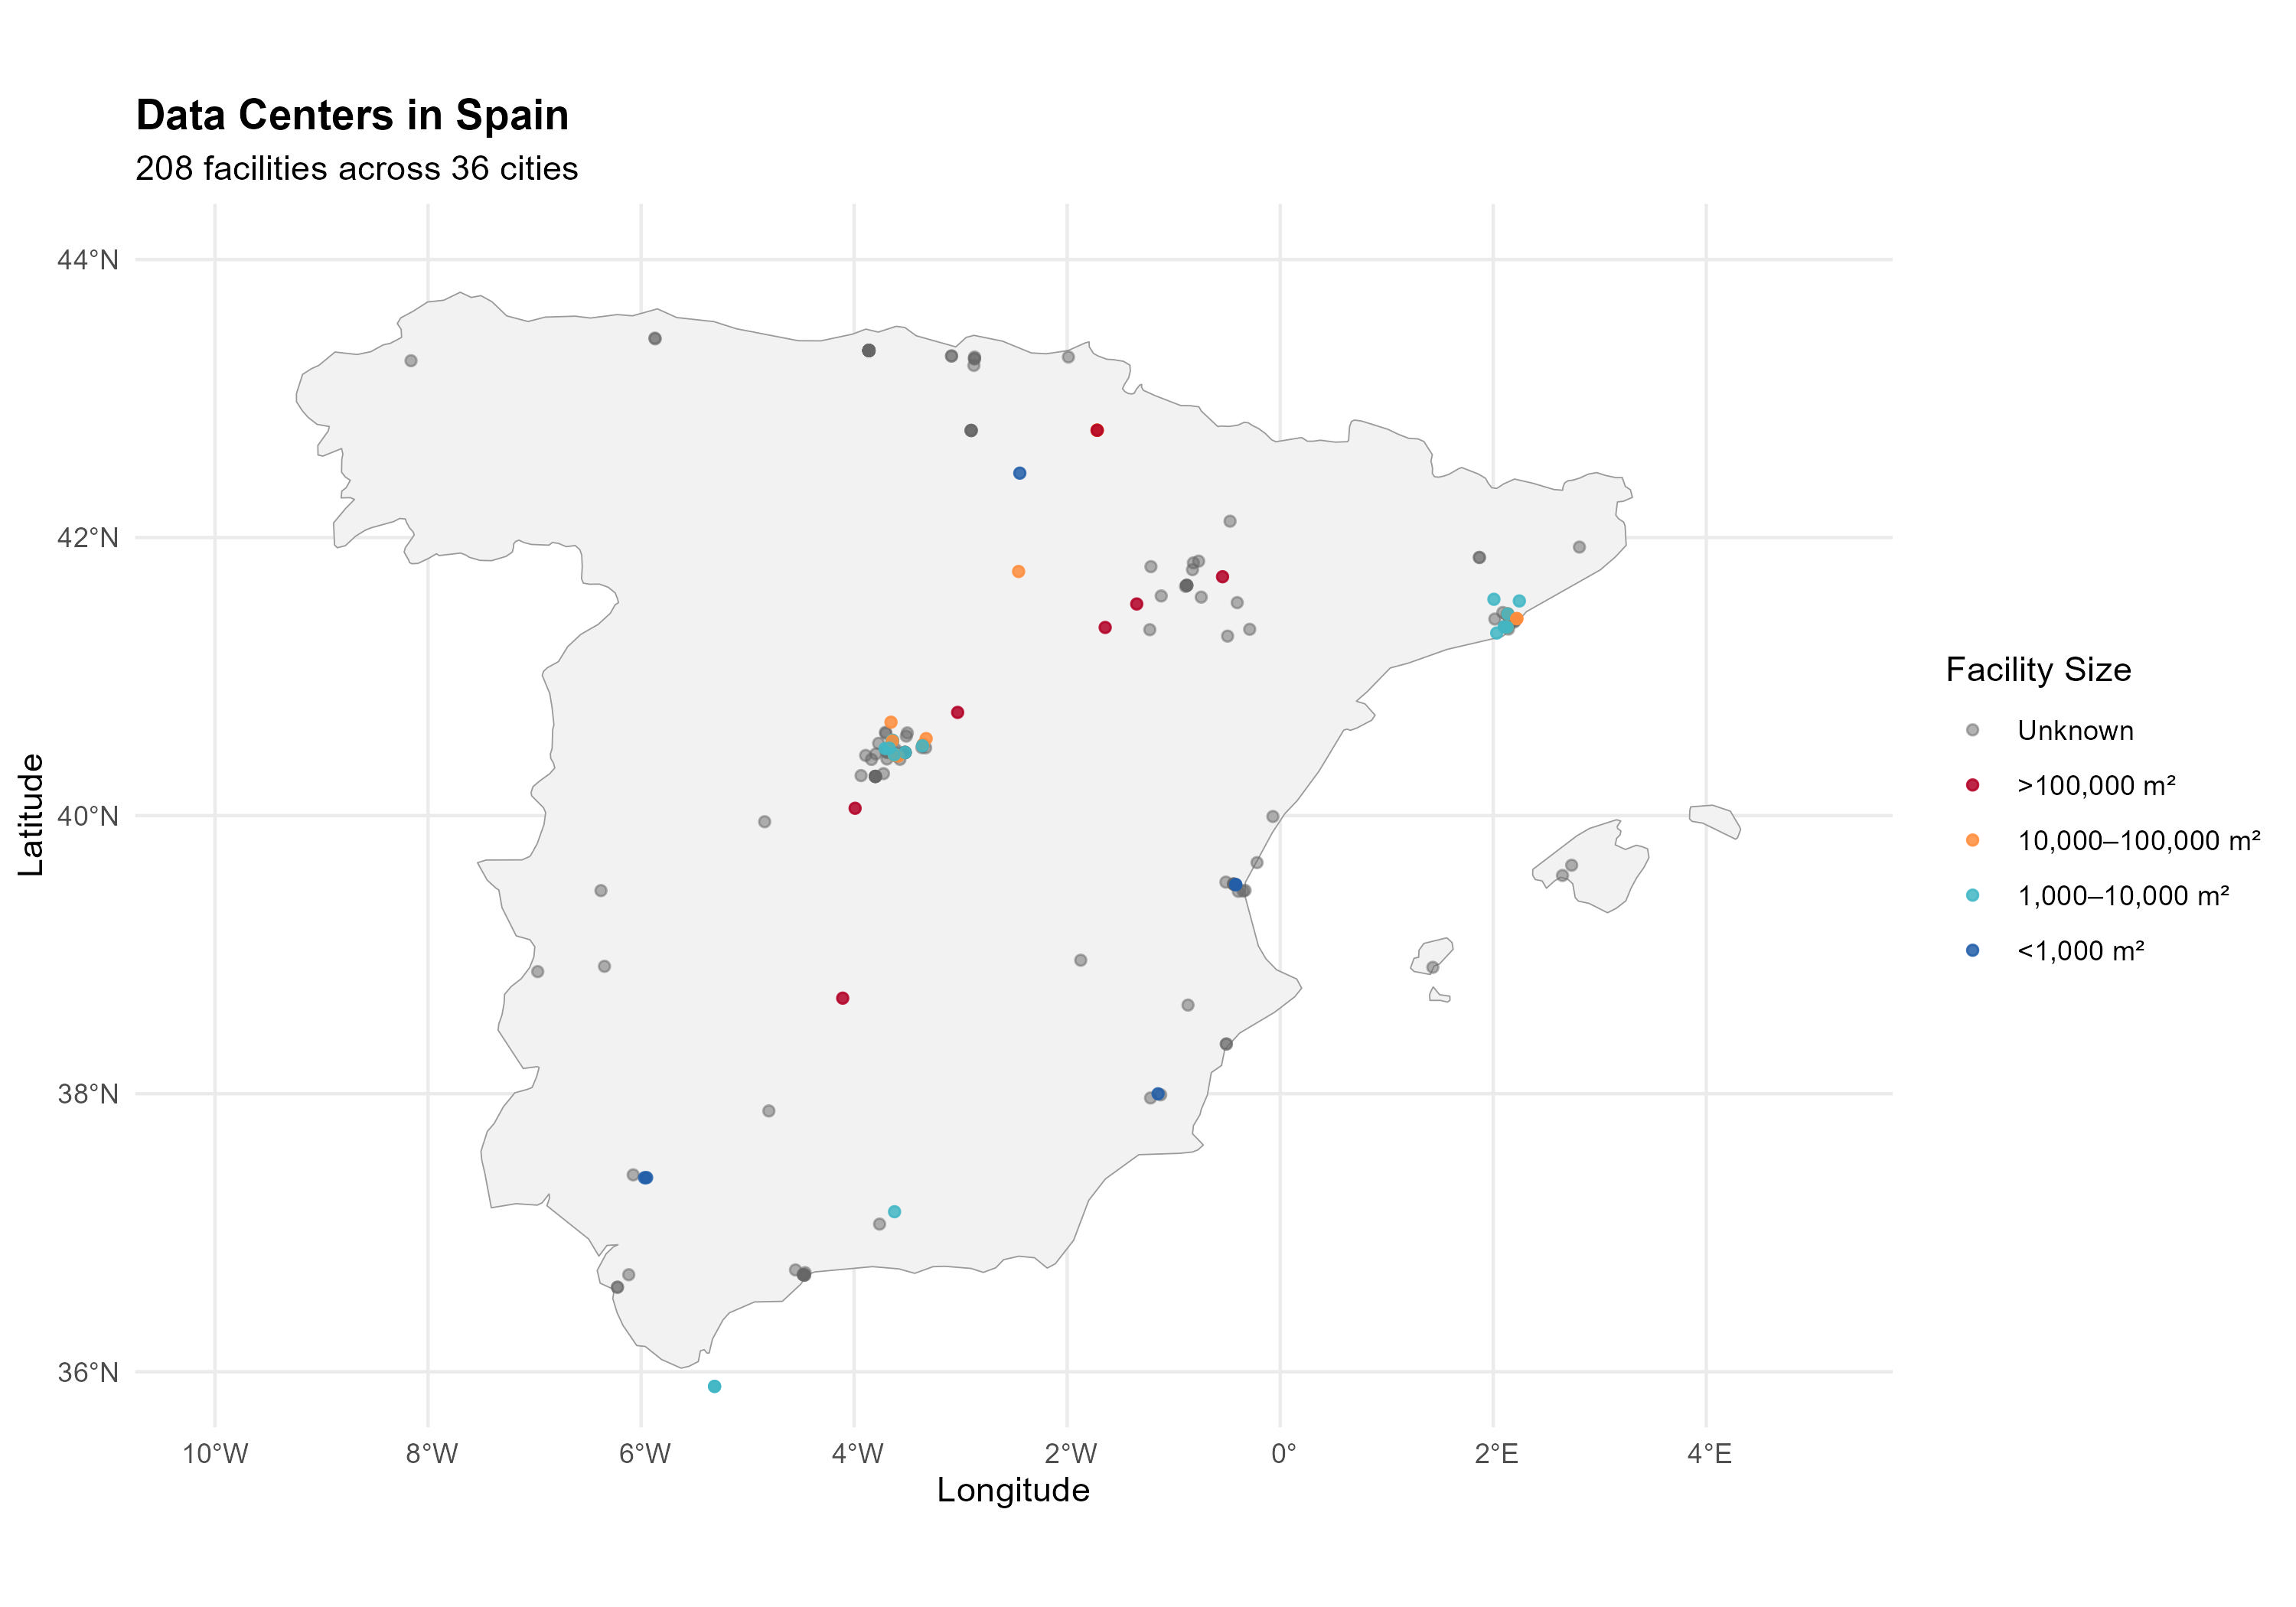
\includegraphics[width=\textwidth]{outputs/data_center_map.jpg}
  \caption{Existing data centers in Spain (from \texttt{DataCenters\_Current\_Map.rmd}). Points are
  colored by facility size category; facilities without size data are shown in black.}
\end{figure}

% Optional Madrid focus map (kept here for reference; remove if not needed)
\begin{figure}[ht]
  \centering
  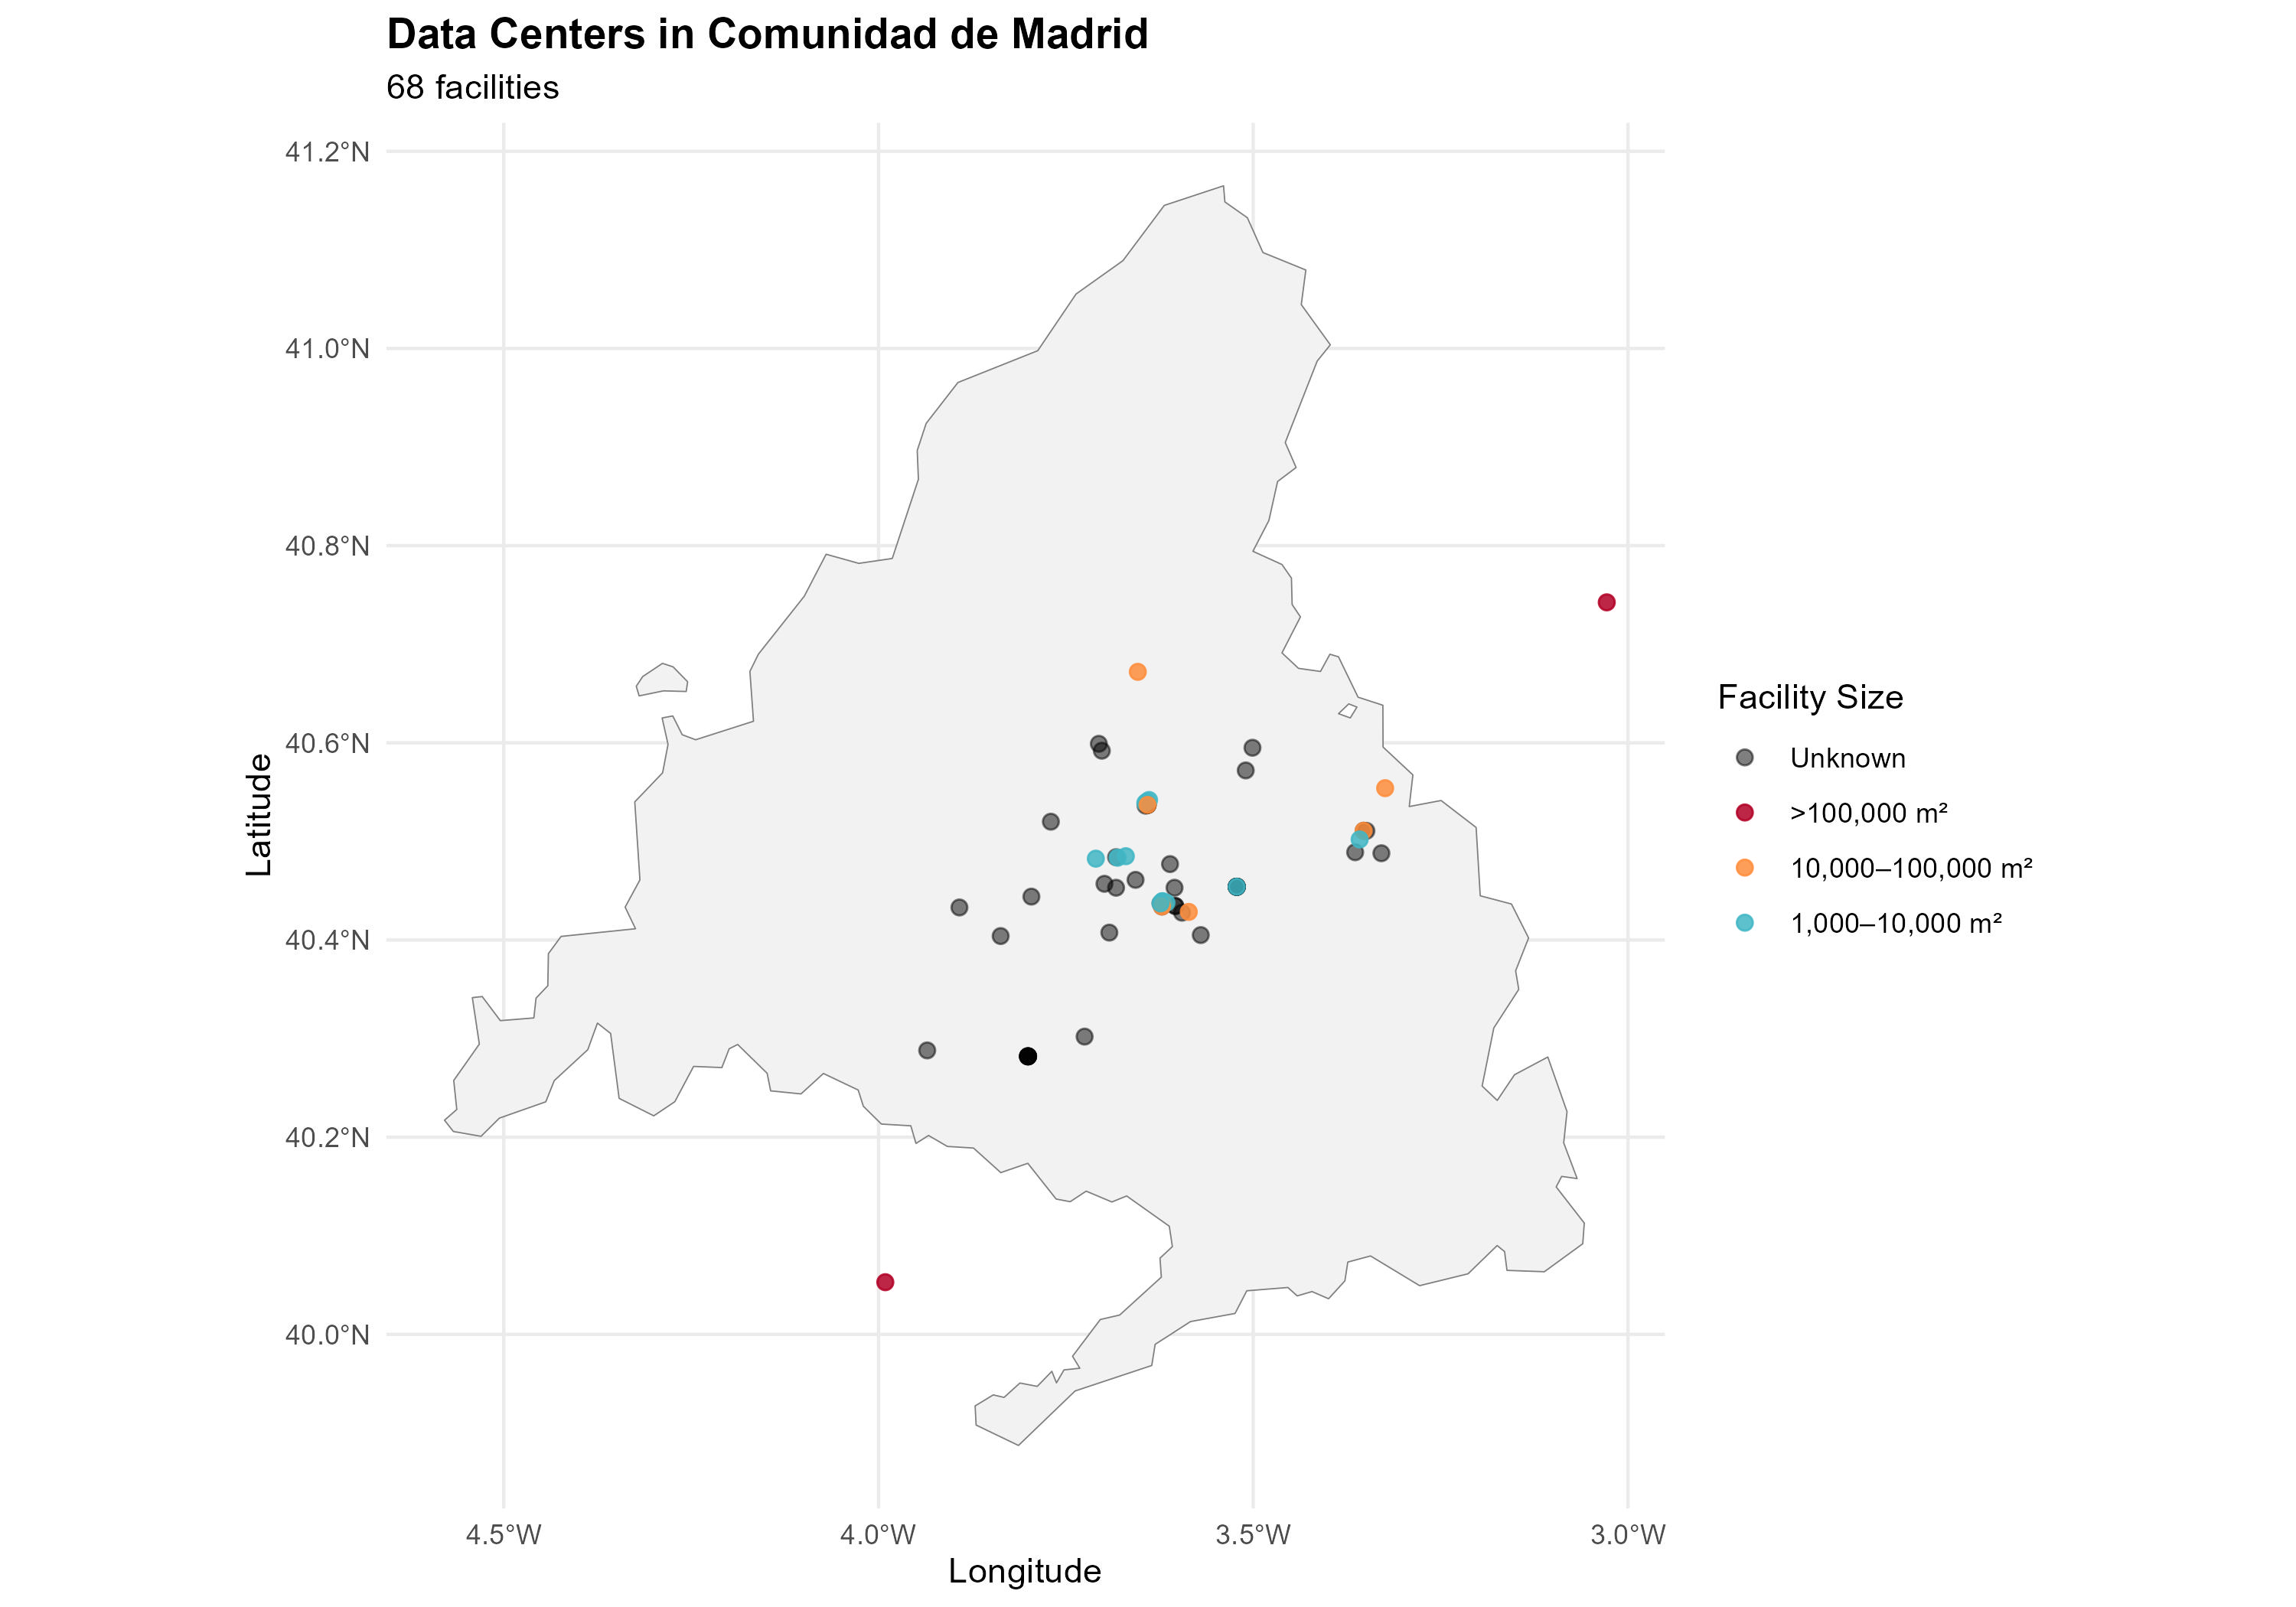
\includegraphics[width=\textwidth]{outputs/madrid_dc_map.jpg}
  \caption{Comunidad de Madrid focus map showing the local concentration of data centers.}
\end{figure}

\section*{Notes for Final Assembly}
\begin{itemize}
  \item Replace the placeholder Map 1 with an exported province boundary map once the GADM/GISCO
  layer is available locally.
  \item If you want this document compiled in Overleaf, ensure the two image files from
  \texttt{outputs/} are uploaded alongside the \texttt{.tex} file.
\end{itemize}

\end{document}
